Let us brieflly retrict our attention to Gaussian measurements for the BPSK coherent-state discrimination problem. As explained in Sec.~\ref{ssec:1_cv_measurements}, such measurements are defined as those that preserve Gaussianity upon post-measurement conditioning or, if the entire state is measured, give rise to Gaussian outcome probability distributions.

A wide class of Guassian measurements are knwon as \textit{general-dyne} measurements, which are POVMs that correspond to projections on generic Gaussian pure states, and discussed in the Preliminaries section. Here, note that such projections might not be orthogonal to each other, as happens in the heterodyne case, \textit{e.g.} projecting over a coherent state, since $\expect{\alpha|\alpha'}\neq0$. Let us also recall that any pure Gaussian state can be obtained through a symplectic unitary operation acting on the vacuum state, and Weyl displacements.

When it comes to discriminate between two Gaussian states, it is known that homodyne POVM (given by projections over quadrature states) is optimal among the set of Gaussian operations~\cite{Limit2021Roberson,opGaussDet, Winter2021Bosonic}. For this reason, homodyne success probability (in the discrimination setting) is known as \textit{the homodyne limit}. Note, nevertheless, that this is subset of all POVMs, and as such it might not saturate the Helstrom bound (see Sec.~\ref{ssec:1_qdisc}). In turn, as mentioned above for the BPSK case, the Helstrom measurement can be attained by projecting over cat-like states, which is a \textit{non-Gaussian} measurement.

\begin{figure}[t!]
    \centering
    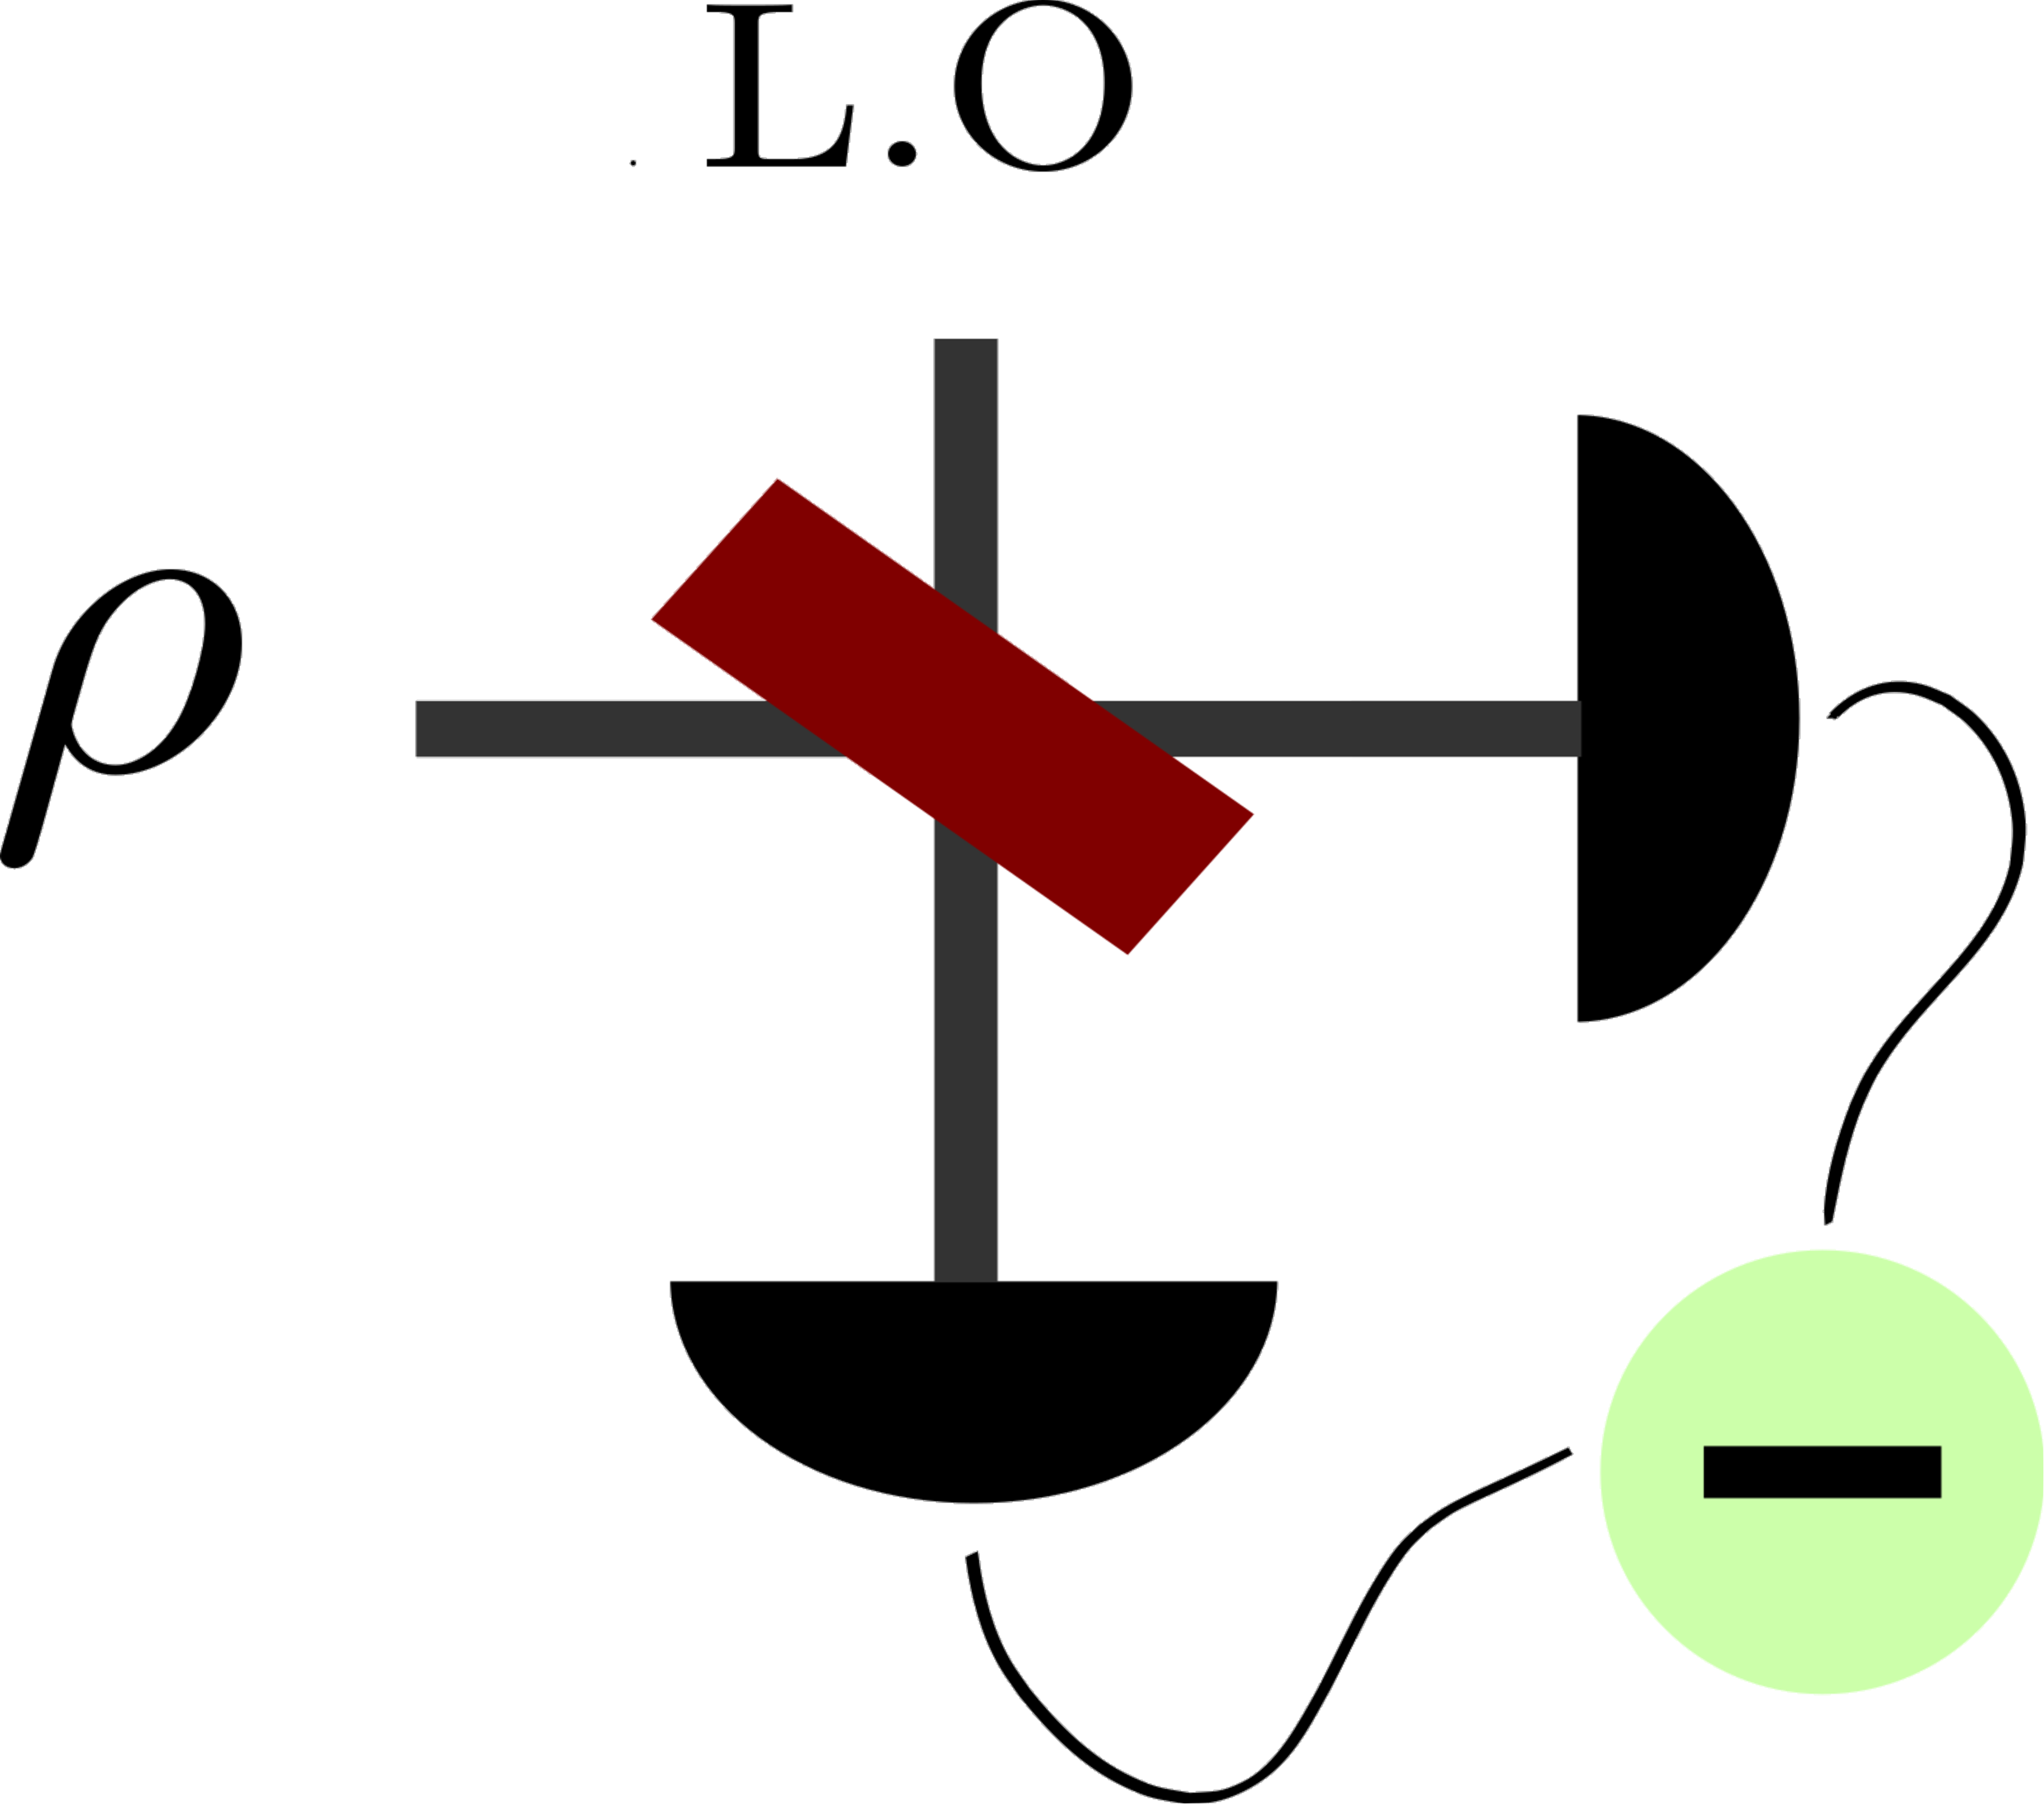
\includegraphics[width=.45\textwidth]{Figures/312/receiver_homodyne.pdf}
    \caption{An implementation of homodyne measurement is shown, which consists on mixing the incoming signal with a coherent state of strong intensity, known as Local Oscillator, by a balanced beam-splitter. The difference in signals' intensities between the two exiting ports constitutes the homodyne measurement outcome~\cite{serafiniBOOK}.}
    \label{fig:homodynereceiver}
\end{figure}

To gain some more insight on the problem, let us derive the success probability attained by homodyne measurement in the BPSK. We consider a quadrature measurement of the form $\mathcal{M} = \llaves{\Pi_-, \Pi_+}$, with $\Pi_- = \int_{-\infty}^{0} dq \ket{q}\bra{q}$, and $\Pi_+= \int_{0}^{\infty} dq \ket{q}\bra{q}$. Given an outcome of the homodyne measurement $q$, the guess for the underlying hypothesis $k$ is chosen according to the sign of $q$: if the value is negative, the signal is associated to $\ket{\alpha^{(1)}} = \ket{-\alpha}$,
whereas if positive to $\ket{\alpha^{(0)}} = \ket{\alpha}$. Such a decision rule is denoted by $\hat{k}(k)$
With this, the success probability reads:
\begin{align}
P_s^{\text{hom}} &= \sum_{k} p_{\hat{k}} p(\hat{k}|k) \\
&= \frac{1}{2} \Big( \int_{-\infty}^0 dq p(q|-\alpha)  +  \int_{0}^\infty dq p(q|+\alpha) \Big)
\end{align}
Recalling that $p(q|\alpha) = |\braket{q}{\alpha}|^2 = \sqrt{\frac{2}{\pi}} e^{2 (q-\alpha)^2}$, a straightforward calculation leads to
\begin{equation}\label{eq:gaussian_receiver_homo}
P_s^{hom} = \frac{1}{2}\big( 1 + \text{Erf}[\sqrt{2} \alpha]\big).
\end{equation}

As shown in Fig.~\ref{fig:homodynereceiver}, the homodyne receiver can be realized by measuring the intensity of the resulting signals after mixing the state $\rho$ with a local oscillator (a high-intensity cohernet state). Quite surprisingly, the building blocks of such standard Gaussian measurement are photon-detectors, which are actually non-Gaussian.

Experimentally, Gaussian operations can be complemented with on/off photon-detectors, constituted by a POVM with elements $\llaves{\Pi_0 = \proj{0}, \Pi_1 = \mathbb{I}-\proj{0}}$, where the $\Pi_1$ is a non-Gaussian projection. Using on-off photon-detections is experimentally feasible, and there has been a trend in the recent years to combine Gaussian transformations with photo-detections carried out by the end of the circuit. While in general one can surpass the homodyne limit, it has been shown that optimality might be elusive in this setting~\cite{nongaussian1}. Before considering more sophisticated receivers, we will now study an example of the aforementioned Gaussian+on/off receiver, named after Kennedy.
%%
